\section{Kopplingsschema}
Robotens elektronik är uppdelad på två virkort. Därför presenteras här ett kopplingsschema för varje virkort.


\nyBild{kopplingsschema_sensor.png}{Kopplingsschema för virkortet som innehåller sensorenheten.}{senskoppling}{1}

\begin{figure}[H]
\centering
 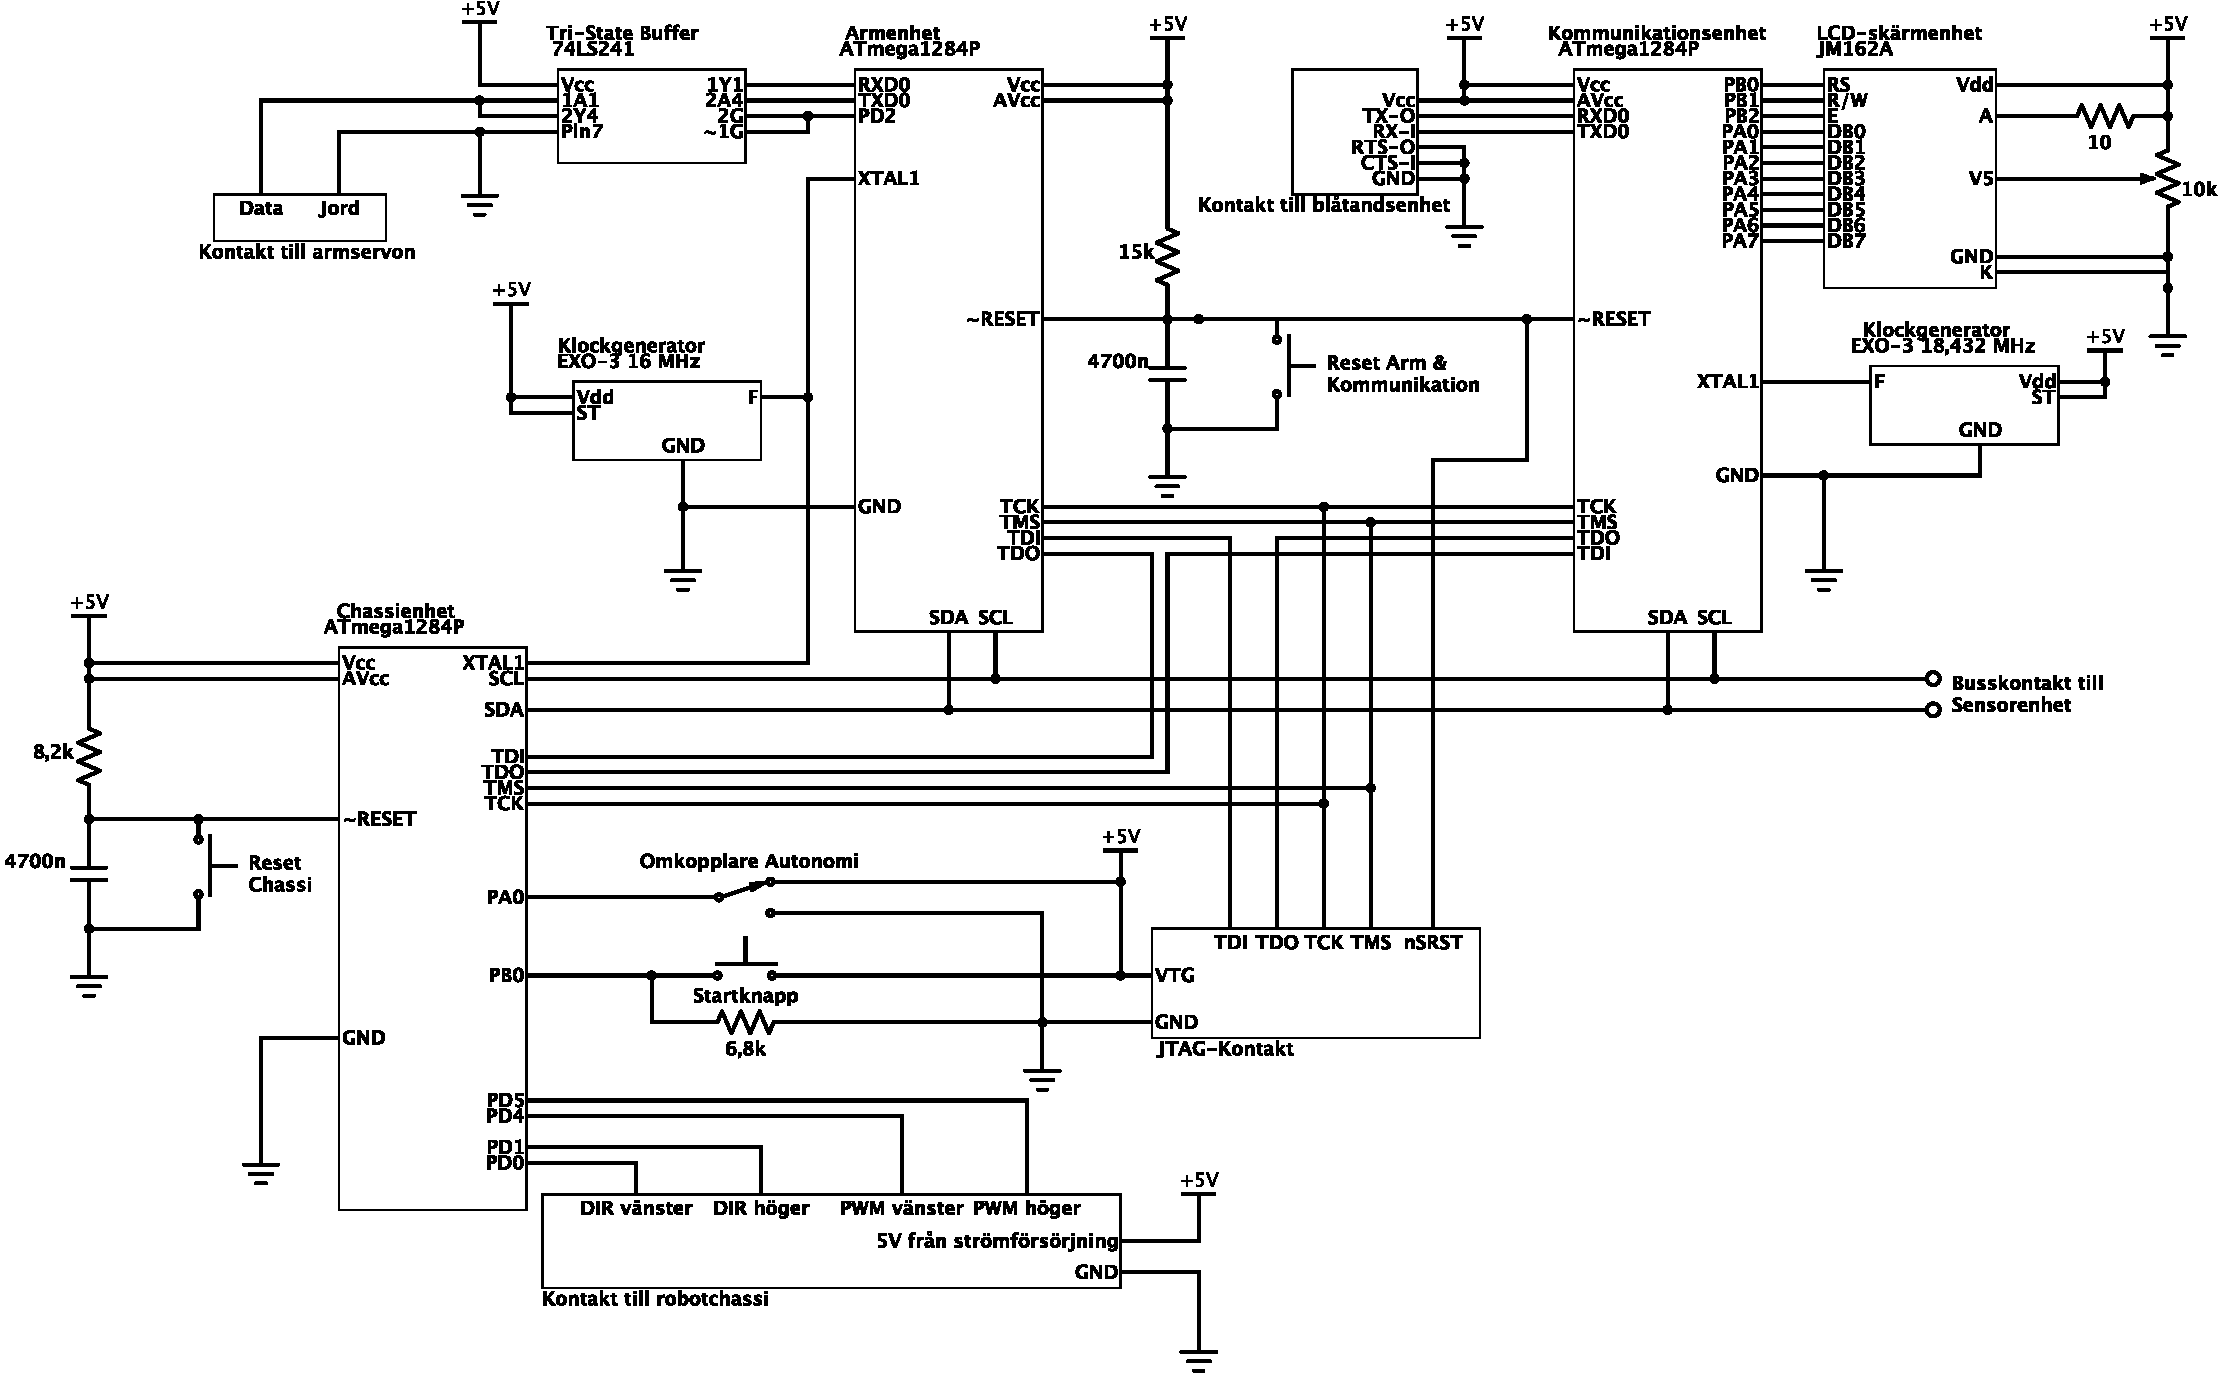
\includegraphics[angle=90,width=0.9\textwidth]{bilder/chassiarmkomm.pdf}
  \emph{\caption{Kopplingsschema över virkortet som innehåller kommunikationsenheten, chassienheten och armenheten.} \label{fig:chassiarmkomm}}
  
\end{figure}


\section{Utdrag från programlistning}
\emph{(ca 5-10 sidor så att vi kan bedöma kodens läsbarhet mm.) och eventuell VHDL-kod}

\section{ID:n till buss}
\label{callbacks}

\begin{table}[H]
\centering
\label{callbacks-sensor}
Delsystem sensor
\begin{tabularx}{\textwidth}{|l|l|X|}
\hline
\textbf{ID} & \textbf{Transaktion/förfrågan} & \textbf{Funktion [data]} \\ \hline
1 & Oanvänd & \\ \hline
2 & Transaktion & Kalibrering av linjesensor \\ \hline
3 & Förfrågan & Linjesensordata \\ \hline
4 & Förfrågan & Tyngpunkt \\ \hline
5 & Transaktion & Sätt tejpreferens [ny tejpreferens] \\ \hline
6 & Oanvänd & \\ \hline
7 & Oanvänd & \\ \hline
8 & Oanvänd & \\ \hline
9 & Transaktion & Sätt aktivitet [0 = linjeföljning, 1 = skanna vänster, 2 = skanna höger] \\ \hline
10 & Transaktion & Läs RFID-tag \\ \hline
\end{tabularx}
\caption{ID:n samt funktion för delsystem sensor}
\end{table}

Delsystem chassi

\begin{table}[H]
\centering
\label{callbacks-chassi}
\begin{tabularx}{\textwidth}{|l|l|X|}
\hline
\textbf{ID} & \textbf{Transaktion/förfrågan} & \textbf{Funktion [data]} \\ \hline
0 & Transaktion & Nödstopp \\ \hline
1 & Oanvänd & \\ \hline
2 & Transaktion & Arm klar [0 = plockat up, 1 = lagt ner, 2 = hittade inget] \\ \hline
3 & Transaktion & Starta linjeföljning \\ \hline
4 & Transaktion & RFID inläst \\ \hline
5 & Oanvänd & \\ \hline
6 & Oanvänd & \\ \hline
7 & Oanvänd & \\ \hline
8 & Transaktion & Uppdatera manuell styrning, se \ref{packets}\\ \hline
9 & Oanvänd & \\ \hline
10 & Oanvänd & \\ \hline
11 & Transaktion & Sätt Kp [nytt värde på Kp] \\ \hline
12 & Transaktion & Sätt Kd [nytt värde på Kd] \\ \hline
\end{tabularx}
\caption{ID:n samt funktion för delsystem chassi}
\end{table}

Delsystem kommunikationsenhet

\begin{table}[H]
\centering
\label{callbacks-komm}
\begin{tabularx}{\textwidth}{|l|l|X|}
\hline
\textbf{ID} & \textbf{Transaktion/förfrågan} & \textbf{Funktion [data]} \\ \hline
1 & Oanvänd & \\ \hline
2 & Transaktion & Rad 1 på skärm för sensorenheten \\ \hline
3 & Transaktion & Rad 2 på skärm för sensorenheten \\ \hline
4 & Transaktion & Rad 1 på skärm för armenheten \\ \hline
5 & Transaktion & Rad 2 på skärm för armenheten \\ \hline
6 & Transaktion & Rad 1 på skärm för chassienheten \\ \hline
7 & Transaktion & Rad 2 på skärm för chassienheten \\ \hline
8 & Transaktion & Vidarebefordra beslut från chassi till PC \\ \hline
9 & Transaktion & Vidarebefordra RFID-tag till PC\\ \hline
10 & Transaktion & Vidarebefordra data från sidoskanner till PC \\ \hline
11 & Transaktion & Sätt Kp [nytt värde på Kp] \\ \hline
12 & Transaktion & Sätt Kd [nytt värde på Kd] \\ \hline
13 & Transaktion & Vidarebefordra kalibreringsvärde till PC \\ \hline
\end{tabularx}
\caption{ID:n samt funktion för delsystem kommunikation}
\end{table}

Delsystem arm

\begin{table}[H]
\centering
\label{callbacks-arm}
\begin{tabularx}{\textwidth}{|l|l|X|}
\hline
\textbf{ID} & \textbf{Transaktion/förfrågan} & \textbf{Funktion [data]} \\ \hline
0 & Transaktion & Nödstopp \\ \hline
1 & Transaktion & Kommando till klo [0 = stäng, 1 = öppna] \\ \hline
2 & Transaktion & Signal att roboten står på station [0 = vänster, 1 = höger] \\ \hline
3 & Transaktion & Vinkel till uppplockning [vinkel] \\ \hline
4 & Transaktion & x koordinat till uppplockning [x] \\ \hline
5 & Transaktion & Plocka upp objekt [0 = inget hittades, 1 = föremål hittat] \\ \hline
6 & Transaktion & x position för manuell styrning [x] \\ \hline
7 & Transaktion & y position för manuell styrning [y] \\ \hline
8 & Transaktion & Vinkel för manuell styrning om positiv [vinkel] \\ \hline
9 & Transaktion & Vinkel för manuell styrning om negativ [vinkel] \\ \hline
10 & Transaktion & Gå till position satt i manuell styrning \\ \hline
11 & Transaktion & Uppdatera manuell styrning, se \ref{packets} \\ \hline
12 & Transaktion & Lämna av objekt [0 = vänster, 1 = höger] \\ \hline
\end{tabularx}
\caption{ID:n samt funktion för delsystem arm}
\end{table}

\section{Protokoll för blåtand}
\begin{table}[H]
\label{packets}
\begin{tabularx}{\textwidth}{|l|X|X|}
\hline
\textbf{ID-beteckning} & \textbf{Beskrivning} & \textbf{Parametrar} \\ \hline
PKT\_STOP & Indikerar att roboten ska stoppa all rörelse. & Inga \\ \hline
PKT\_ARM\_COMMAND & Kommando till arm. & Kommando (1), argument (2-10) \\ \hline
PKT\_CHASSIS\_COMMAND & Kommando till chassi. & Kommando (1), argument (2-3) \\ \hline
PKT\_CALIBRATION\_COMMAND & Kommando för klibrering av sensor. & Sensor id (1) \\ \hline
PKT\_LINE\_DATA & Data från linjesensorn. & Inviduella sensorer (1-11), flaggor (12), tyngdpunkt (13), styrutslag (14) \\ \hline
PKT\_RANGE\_DATA & Avstånd från sidoskanner. & sida (1), avstånd (2-3) \\ \hline
PKT\_RFID\_DATA & Värde på RFID-tagg & värde (1) \\ \hline
PKT\_CHASSIS\_DECISION & Beslut från chassi. & beslut (1) \\ \hline
PKT\_PACKET\_REQUEST & Förfrågan om paket från dator. & ID på packet (1) \\ \hline
PKT\_SPOOFED\_RESPONSE & Simulerad förfågran på bussen. & Data som skickas ut på bussen (1-2) \\ \hline
PKT\_SPOOFED\_TRANSMIT & Simulerad transmitt på bussen. & Data som skickas ut på bussen. (1-2) \\ \hline
PKT\_CALIBRATION\_DATA & Värde efter kalibrering. & Värde (1) \\ \hline
PKT\_LINE\_WEIGHT & Tyngpunkt från linjesensor. & Tyngdpunkt (1) \\ \hline
\end{tabularx}
\caption{De olika pakettyper som kan skickas mellan roboten och PC och vad de innehåller. Parametrarnas ordningsnummer i parameterföljden anges inom parentes i den sista kolumnen.}
\end{table}

\begin{table}[H]
\label{commands}
\begin{tabularx}{\textwidth}{|l|X|X|}
\hline
\textbf{ID-beteckning} & \textbf{Beskrivning} & \textbf{Parametrar} \\ \hline
CMD\_ARM\_MOVE & Arm ska röra sig. & Koordinat (1), riktning (2) \\ \hline
CMD\_ARM\_GRIP & Stäng gripklo. & Inga \\ \hline
CMD\_ARM\_RELEASE & Öppna gripklo. & Inga \\ \hline
CMD\_ARM\_PREDEFINED\_POS & Rör arm till fördefinerad position. & ID på position \\ \hline
CMD\_ARM\_STOP & Stanna alla rörelser. & Inga \\ \hline
CMD\_ARM\_MOVE\_POS & Rör arm till position. & x (1), y (2), vinkel (3) \\ \hline
CMD\_CHASSIS\_SPEED & Ny hastighet till chassi. & Hastighet (1) \\ \hline
CMD\_CHASSIS\_STEER & Sätt nytt rattutslag. & Rattutslag (1) \\ \hline
CMD\_CHASSIS\_START & Starta linjeföljning. & Inga \\ \hline
CMD\_CHASSIS\_PARAMETERS & Sätt nya värde på $K_p$ och $K_d$. & $K_p$(1), $K_d$(2) \\ \hline
CMD\_CHASSIS\_MOVEMENT & Kommando till chassi att röra på sig i en given riktning. & Riktning (1) \\ \hline
\end{tabularx}
\caption{De olika pakettyper som kan skickas mellan roboten och PC och vad de innehåller. Parametrarnas ordningsnummer i parameterföljden anges inom parentes i den sista kolumnen.}
\end{table}

\begin{table}[H]
\label{decision}
\begin{tabularx}{\textwidth}{|l|l|X|}
\hline
\textbf{ID-beteckning} & \textbf{Beskrivning} & \textbf{Parametrar} \\ \hline
DEC\_PICKUP\_RIGHT & Plockar upp föremål höger. & Inga \\ \hline
DEC\_PICKUP\_LEFT & Plockar upp föremål vänster. & Inga \\ \hline
DEC\_PUT\_DOWN\_RIGHT & Lägger ner föremål höger. & Inga \\ \hline
DEC\_PUT\_DOWN\_LEFT & Lägger ner föremål vänster. & Inga \\ \hline
DEC\_NO\_MATCH & RFID var inte korrekt. & Inga \\ \hline
DEC\_STATION\_HANDELED & Station redan behandlad. & Inga \\ \hline
DEC\_NO\_ID\_FOUND & Ingen RFID-tagg hittade på stationen. & Inga \\ \hline
DEC\_ARM\_PICKED\_UP & Arm har plockat upp ett föremål. & Inga \\ \hline
DEC\_ARM\_PUT\_DOWN & Arm har lagt ned ett föremål. & Inga \\ \hline
DEC\_OBJECT\_NOT\_FOUND & Inget föremål hittades. & Inga \\ \hline
DEC\_UNKOWN\_ERROR & Okänt fel inträffade. & Inga \\ \hline
DEC\_ARM\_FAILED & Arm misslyckades med uppplockning. & Inga \\ \hline
DEC\_START\_LINE & Startade linjeföljning. & Inga \\ \hline
\end{tabularx}
\caption{De olika pakettyper som kan skickas mellan roboten och PC och vad de innehåller. Parametrarnas ordningsnummer i parameterföljden anges inom parentes i den sista kolumnen.}
\end{table}

\section{Övriga bilagor?}
